\documentclass[Master,ngerman,UKenglish,twoside]{scrbook}
%------------------------------------------------------------------------------
% This file contains a skeleton thesis for
% a Physics or Astronomy Institute in the University of Bonn

% Specify the thesis type as an option: PhD, Master, Diplom, Bachelor
% Specify the thesis stage as an option: Draft (default), Submit, Final, PILibrary

% Specify the language(s) in the class and then use babel.
% If you need more than one language, give the default language last,
% e.g. ngerman,UKenglish for a thesis in British (UK) English where you want
% to be able to set the language to German for some part of it.

%------------------------------------------------------------------------------
% Pass TeX Live version to the package
% Use command pdflatex --version to find out which version you are running
% Add option backref=false when your thesis is ready to turn off back-referencing
% in your bibliography



\usepackage[texlive=2014]{ubonn-thesis}
% Adjustments to standard biblatex style


\usepackage[backend=biber,style=numeric-comp,sorting=none,block=ragged,firstinits=true]{biblatex}

\usepackage{ubonn-biblatex}

\addbibresource{thesis_refs.bib}
%\addbibresource{../refs/standard_refs-biber.bib}






% Glossary package
% \usepackage[acronym,toc,nosuper]{glossaries}
% TikZ packages and libraries
\usepackage{tikz}
 \usepackage{tikz-3dplot}
 \usepackage{pgfplots}
 \usetikzlibrary{positioning,shapes,arrows}
 \usetikzlibrary{decorations.pathmorphing}
 \usetikzlibrary{decorations.markings}
\usepackage{thesis_defs}
%\usepackage{tikz}
\usetikzlibrary{calc,positioning,shadows.blur,decorations.pathreplacing}
\usepackage{etoolbox}
\usepackage{verbatim}
%%%>

\tikzset{%
	brace/.style = { decorate, decoration={brace, amplitude=5pt} },
	mbrace/.style = { decorate, decoration={brace, amplitude=5pt, mirror} },
	label/.style = { black, midway, scale=0.5, align=center },
	toplabel/.style = { label, above=.5em, anchor=south },
	leftlabel/.style = { label,rotate=-90,left=.5em,anchor=north },   
	bottomlabel/.style = { label, below=.5em, anchor=north },
	force/.style = { rotate=-90,scale=0.4 },
	round/.style = { rounded corners=2mm },
	legend/.style = { right,scale=0.4 },
	nosep/.style = { inner sep=0pt },
	generation/.style = { anchor=base }
}

%------------------------------------------------------------------------------
% Instead of colouring  links, cites, table of contents etc.
% put them in a coloured box for the screen version.
% This is probably a good idea when you print your thesis.
% \hypersetup{colorlinks=false,
%   linkbordercolor=blue,citebordercolor=magenta,urlbordercolor=darkgreen
% }

%------------------------------------------------------------------------------
% When writing your thesis it is often helpful to have the date and
% time in the output file. Comment this out for the final version.
\ifoot[\today{} \thistime]{\today{} \thistime}

% In order to check if your labels are referenced try the refcheck package
% \usepackage{refcheck}




%------------------------------------------------------------------------------
% biblatex is included by ubonn-thesis. Look there for the settings used.
% See the options for settings that can be changed easily.
% For further changes copy the \RequirePackage[...]{biblatex} here
% and include ubonn-thesis with the option biblatex=false.

% Specify the bibliography files here and not at the end!
% Use standard_refs-bibtex if you use bibtex or bibtex8
% and standard_refs-biber  if you use biber
\addbibresource{thesis_refs.bib}
%\addbibresource{../refs/standard_refs-biber.bib}

%------------------------------------------------------------------------------
% The following definitions are used to produce the title pages
% needed at various stages
%%\newcommand{\thesistitle}{Title of the Thesis}
%%\newcommand*{\thesisauthor}{Author's name}
%%\newcommand*{\thesistown}{Place of birth}
%%\renewcommand*{\InstituteName}{\PI}
%%\renewcommand*{\inInstitute}{\inPI}
%%\renewcommand*{\InstituteAddress}{\PIaddress}
% Adjust \thesisreferee...text depending on male/female referee
%%\newcommand*{\thesisrefereeonetext}{1.\ Gutachter}
%%\newcommand*{\thesisrefereeone}{Prof.\ Dr.\ John Smith}
%%\newcommand*{\thesisrefereetwotext}{2.\ Gutachterin}
%%\newcommand*{\thesisrefereetwo}{Prof.\ Dr.\ Anne Jones}
% Date when thesis was submitted (Master/Diplom)
% Year or Month, Year when thesis was submitted (PhD)
%%\newcommand*{\thesissubmit}{XX.YY.2016}
% \newcommand*{\thesissubmit}{Month 2016}
% Date of thesis examination (PhD)
%%\newcommand*{\thesispromotion}{XX.YY.2016}
% Month and year of the final printed version of the thesis
%%\newcommand*{\thesismonth}{MMM}
%%\newcommand*{\thesisyear}{2016}
%%\newcommand*{\thesisnumber}{BONN-IR-2016-XXX}

%------------------------------------------------------------------------------
% The abstract is only needed for the printed version and should be in
% English regardless of the language of the thesis
\newcommand{\thesisabstract}{%
  \begin{otherlanguage}{UKenglish}
    This is your thesis abstract. It may be in a language that is
    different from the rest of your thesis.
  \end{otherlanguage}
}

%------------------------------------------------------------------------------
% \includeonly can be used to select which chapters you want to process
% A simple \include command just inserts a \clearpage before and after the file
% Note that \includeonly can be quite picky! Do not forget to put a
% comma after the filename, otherwise it will simply be ignored!
% \includeonly{%
%   thesis_intro,
%   thesis_appendix,
%   thesis_acknowledge
% }

%------------------------------------------------------------------------------
% Give a list of directories where figures can be found. Do not leave
% any spaces in the list and end the directory name with a /
\graphicspath{%
  {../figs/}%
  {../figs/cover/}%
  {../figs/graphics/}%
  {../feynmf/}%
}

%------------------------------------------------------------------------------
% Make a glossary and a list of acronyms
% \makeglossaries

% Glossary entries
% \input{thesis_glossary}

% Draft version - add the word DRAFT on the cover pages

%\ifthenelse{\equal{\ThesisVersion}{Draft}}{%
 %
 %\usepackage{background}
  %\ifthenelse{\texlive < 2013}{%
   % \SetBgContents{DRAFT}
    %\SetBgColor{blue!30}
  %}{%
%    \backgroundsetup{contents=DRAFT, color=blue!30}
 % }
%}



\usepackage{hyperref}
\usepackage[english]{cleveref}

%------------------------------------------------------------------------------
\begin{document}

% Cover page of thesis - this is only needed for the printed final
% version to be submitted to the department library
% Do not use this page for thesis submission to the Prüfungsamt or Promotionsbüro!
\ifthenelse{\equal{\ThesisVersion}{PILibrary}}{%
  \typeout{Document \jobname, Info: PI library version of thesis}
 % \input{../cover/\ThesisType_Cover}
}{}

% Start counting pages from the title page
\frontmatter
% Dedication has to come before \maketitle
% \dedication{For ...}

% Select the correct title page(s)
\ifthenelse{\equal{\ThesisType}{Unknown}}{%
  \typeout{Document \jobname, Error: Unknown thesis type - no title page printed}
}{%
  % Bachelor thesis only has one title page
  \ifthenelse{\equal{\ThesisType}{Bachelor}}{%
    \typeout{Document \jobname, Info: Bachelor thesis}
    %\input{../cover/\ThesisType_Title}
  }{%
    \ifthenelse{\equal{\ThesisVersion}{Final} \OR \equal{\ThesisVersion}{PILibrary}}{%
      % Final and PI library versions
      \typeout{Document \jobname, Info: Final version of a \ThesisType  thesis}
      %\input{../cover/\ThesisType_Final_Title}
    }{% Submission and draft versions
     % \input{../cover/\ThesisType_Submit_Title}
      \typeout{Document \jobname, Info: Draft/submission version of a \ThesisType  thesis}
    }
  }
}

\pagestyle{scrplain}

%------------------------------------------------------------------------------
% You can add your acknowledgements here - don't forget to also add
% them to \includeonly above
%%------------------------------------------------------------------------------
\chapter*{Acknowledgements}
\label{sec:ack}
%------------------------------------------------------------------------------

I would like to thank ...

You should probably use \texttt{\textbackslash chapter*} for
acknowledgements at the beginning of a thesis and
\texttt{\textbackslash chapter} for the end.

%%% Local Variables: 
%%% mode: latex
%%% TeX-master: "../mythesis"
%%% End: 


\tableofcontents

\mainmatter
\pagestyle{scrheadings}

% Turn off DRAFT for the following pages
%\ifthenelse{\equal{\ThesisVersion}{Draft}}{%
  %\ifthenelse{\texlive < 2013}{%
   % \SetBgContents{}
  %}{%
  %  \backgroundsetup{contents={}}
 % }
%}{}

%------------------------------------------------------------------------------
% Add your chapters here - don't forget to also add them to \includeonly above
\chapter{Introduction}

\label{sec:intro}
%==============================================================================

The introduction usually gives a few pages of introduction to the
whole subject, maybe even starting with the Greeks.

For more information on \LaTeX{} and the packages that are available
see for example the books of Kopka~\cite{kopka04} and Goossens et
al~\cite{goossens04}.

A lot of useful information on particle physics can be found in the
\enquote{Particle Data Book}~\cite{pdg2010}.

I have resisted the temptation to put a lot of definitions into the
file \texttt{thesis\_defs.sty}, as everyone has their own taste as
to what scheme they want to use for names.
However, a few examples are included to help you get started:
\begin{itemize}
\setlength{\itemsep}{0pt}\setlength{\parskip}{0pt}
\item cross-sections are measured in \si{\pb} and integrated
  luminosity in \si{\invpb};
\item the \KoS is an interesting particle;
\item the missing transverse momentum, \pTmiss, is often called
  missing transverse energy, even though it is calculated using a vector sum.
\end{itemize}
Note that the examples of units assume that you are using the
\textsf{siunitx} package.

It also is probably a good idea to include a few well formatted
references in the thesis skeleton. More detailed suggestions on what
citation types to use can be found in the thesis
guide~\cite{thesis-guide}:
\begin{itemize}
\item articles in refereed journals\cite{pdg2010,Aad:2010ey};
\item a book~\cite{Halzen:1984mc};
\item a PhD thesis~\cite{tlodd:2012} and a Diplom thesis~\cite{mergelmeyer:2011};
\item a collection of articles~\cite{lhc:vol1};
\item a conference note~\cite{ATLAS-CONF-2011-008};
\item a preprint~\cite{atlas:perf:2009} (you can also use
  \texttt{@online} or \texttt{@booklet}for such things;
\item something that is only available online~\cite{thesis-guide}.
\end{itemize}

At the end of the introduction it is normal to say briefly what comes
in the following chapters.

The lines at the end of this file are used by AUCTeX to specify which
is the master \LaTeX{} file, so that you can compile your thesis
directly within \texttt{emacs}.


At the end of the introduction it is normal to say briefly what comes
in the following chapters.

The lines at the end of this file are used by AUCTeX to specify which
is the master \LaTeX{} file, so that you can compile your thesis
directly within \texttt{emacs}.

At the end of the introduction it is normal to say briefly what comes
in the following chapters.

The lines at the end of this file are used by AUCTeX to specify which
is the master \LaTeX{} file, so that you can compile your thesis
directly within \texttt{emacs}.

At the end of the introduction it is normal to say briefly what comes
in the following chapters.

The lines at the end of this file are used by AUCTeX to specify which
is the master \LaTeX{} file, so that you can compile your thesis
directly within \texttt{emacs}.

At the end of the introduction it is normal to say briefly what comes
in the following chapters.

The lines at the end of this file are used by AUCTeX to specify which
is the master \LaTeX{} file, so that you can compile your thesis
directly within \texttt{emacs}.

At the end of the introduction it is normal to say briefly what comes
in the following chapters.

The lines at the end of this file are used by AUCTeX to specify which
is the master \LaTeX{} file, so that you can compile your thesis
directly within \texttt{emacs}.



j

%%% Local Variables: 
%%% mode: latex
%%% TeX-master: "../mythesis"
%%% End: 

%------------------------------------------------------------------------------
\chapter{The Standard Model of Partical Physics}
\label{sec:SM}
%------------------------------------------------------------------------------
The basic principal behinde the interactions, which are mediated by gauge Bosons, is  that the Lagrange density is invariant under local gauge transformation. More Precisse, the particals are discribed as Fields. The Time and Space evolution of those fields follows the Euler-Lagrange equation which can be determinde using Hamiltions variation Pricipall of minmal Action. 
Loclal gauge trenasoformation
The basic principal behinde the interactions, which are mediated by gauge Bosons, is  that the Lagrange density is invariant under local gauge transformation. More Precisse, the particals are discribed as Fields. The Time and Space evolution of those fields follows the Euler-Lagrange equation which can be determinde using Hamiltions variation Pricipall of minmal Action. 
Loclal gauge trenasoformation




\section{Fundamental  Particals, Fields and Forces }\label{key:SM 2}

The Standard Modell of Partical Physics \cite{glashow1961partial,glashow1970weak,gross1973asymptotically,politzer1973reliable,politzer1974asymptotic,salam1964electromagnetic,weinberg1967model}, is a re-normalizable and relativistic Quantum Field Theory (QFT) of the fundamental fermions (spin $s =1/2$) and their interactions mediated by gauge bosons (spin $s = 1$).  It is based on a small number of particles and symmetry principles. Basically, as shown in \cref{fig:SM}, there are three fermion generations. Each of them consists of  a up- and a down type quark, a charged lepton and a corresponding neutrino. \\ 

It's basic structure is depicted in   , with three generations of fermions (quarks and leptons), of which each conists of a up- and a down type quark, a charged lepton and a corresponding neutrino.  The existence of further heavy  generation of up- and down-type has been exluded as for Mt and Mb wit 95 CL.
Additionally the mass of a possible 4th lepton generation is limmited by the mass of the Z boson, and its lifetime Measuremntes confirms only three light neutrion generatis. \\ 





In the theory the particles are described as fields $\psi$, which follow 

\noindent The basic principal behinde the interactions, which are mediated by gauge Bosons, is  that the Lagrange density is invariant under local gauge transformation. More Precisse, the particals are discribed as Fields. The Time and Space evolution of those fields follows the Euler-Lagrange equation which can be determinde using Hamiltions variation Pricipall of minmal Action. 
Loclal gauge trenasoformation
%based on a small number of fields and symetrieprinciels  



Local gauge invariance requires the Standard Model Lagrangian to remain invariant when transforming the fermion fields in the following manner:
ψ → ψ exp(−iα j(x) f j). (2.1)
This principle is only valid in the presence of (massless) fields which transform in the same manner as the fermion fields thus compensating the fermion field transformations in each point of space and time. Based on the choice of the local gauge symmetry group the strong and electroweak interaction theories emerge - introducing a set of bosonic particles intermediating the corresponding forces. Following Noether’s theorem, each symmetry group introduces field-charges which are conserved under local gauge transfromation.




% Standard model of physics
% Author: Carsten Burgard

%%%<


\begin{figure}
	\centering



\newcommand\particle[7][white]{%
	\begin{tikzpicture}[x=1cm, y=1cm]
	\path[fill=#1,] (0.1,0) -- (0.9,0)
	arc (90:0:1mm) -- (1.0,-0.9) arc (0:-90:1mm) -- (0.1,-1.0)
	arc (-90:-180:1mm) -- (0,-0.1) arc(180:90:1mm) -- cycle;
	\ifstrempty{#7}{}{\path[]
		(0.6,0) --(0.7,0) -- (1.0,-0.3) -- (1.0,-0.4);}
	\ifstrempty{#6}{}{\path[] (0.7,0) -- (0.9,0)
		arc (90:0:1mm) -- (1.0,-0.3);}
	\ifstrempty{#5}{}{\path[] (1.0,-0.7) -- (1.0,-0.9)
		arc (0:-90:1mm) -- (0.7,-1.0);}
	\draw[\ifstrempty{#2}{dashed}{black}] (0.1,0) -- (0.9,0)
	arc (90:0:1mm) -- (1.0,-0.9) arc (0:-90:1mm) -- (0.1,-1.0)
	arc (-90:-180:1mm) -- (0,-0.1) arc(180:90:1mm) -- cycle;
	\ifstrempty{#7}{}{\node at(0.825,-0.175) [rotate=-45,scale=0.2] {#7};}
	\ifstrempty{#6}{}{\node at(0.9,-0.1)  [nosep,scale=0.17] {#6};}
	\ifstrempty{#5}{}{\node at(0.9,-0.9)  [nosep,scale=0.2] {#5};}
	\ifstrempty{#4}{}{\node at(0.1,-0.1)  [nosep,anchor=west,scale=0.25]{#4};}
	\ifstrempty{#3}{}{\node at(0.1,-0.85) [nosep,anchor=west,scale=0.3] {#3};}
	\ifstrempty{#2}{}{\node at(0.1,-0.5)  [nosep,anchor=west,scale=1.5] {#2};}
	\end{tikzpicture}
}


	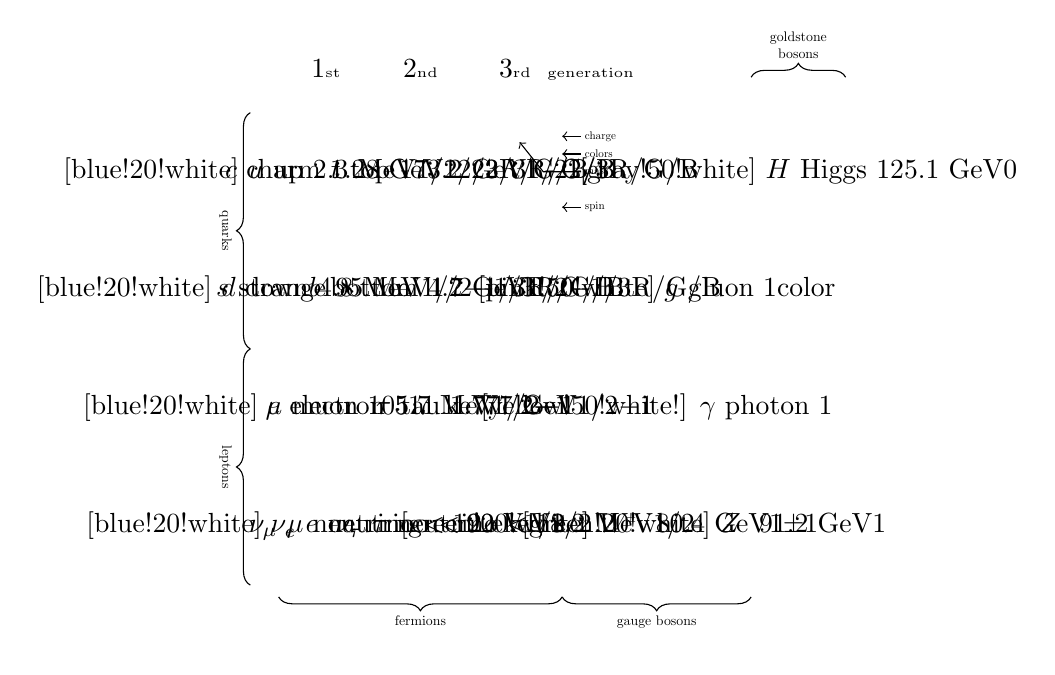
\begin{tikzpicture}[x=1.2cm, y=1.5cm]
	%\draw (-0.5,0.5) rectangle (4.4, -1.5);
	%\draw (-0.6,0.6) rectangle (5.0,-2.5);
	%\draw (-0.7,0.7) rectangle (5.6,-3.5);
	
	\node at(0, 0)   {\particle[blue!20!white]
		{$u$}        {up}       {$2.3$ MeV}{1/2}{$2/3$}{R/G/B}};
	\node at(0,-1)   {\particle[blue!20!white]
		{$d$}        {down}    {$4.8$ MeV}{1/2}{$-1/3$}{R/G/B}};
	\node at(0,-2)   {\particle[blue!20!white]
		{$e$}        {electron}       {$511$ keV}{1/2}{$-1$}{}};
	\node at(0,-3)   {\particle[blue!20!white]
		{$\nu_e$}    {$e$ neutrino}         {$<2$ eV}{1/2}{}{}};
	\node at(1, 0)   {\particle
		{$c$}        {charm}   {$1.28$ GeV}{1/2}{$2/3$}{R/G/B}};
	\node at(1,-1)   {\particle 
		{$s$}        {strange}  {$95$ MeV}{1/2}{$-1/3$}{R/G/B}};
	\node at(1,-2)   {\particle
		{$\mu$}      {muon}         {$105.7$ MeV}{1/2}{$-1$}{}};
	\node at(1,-3)   {\particle
		{$\nu_\mu$}  {$\mu$ neutrino}    {$<190$ keV}{1/2}{}{}};
	\node at(2, 0)   {\particle
		{$t$}        {top}    {$173.2$ GeV}{1/2}{$2/3$}{R/G/B}};
	\node at(2,-1)   {\particle
		{$b$}        {bottom}  {$4.7$ GeV}{1/2}{$-1/3$}{R/G/B}};
	\node at(2,-2)   {\particle
		{$\tau$}     {tau}          {$1.777$ GeV}{1/2}{$-1$}{}};
	\node at(2,-3)   {\particle
		{$\nu_\tau$} {$\tau$ neutrino}  {$<18.2$ MeV}{1/2}{}{}};
	\node at(3,-3)   {\particle[green!20!white]
		{$W^{\hspace{-.3ex}\scalebox{.5}{$\pm$}}$}
		{}              {$80.4$ GeV}{1}{$\pm1$}{}};
	\node at(4,-3)   {\particle[green!20!white]
		{$Z$}        {}                    {$91.2$ GeV}{1}{}{}};
	\node at(3.5,-2) {\particle[yellow!50!white!]
		{$\gamma$}   {photon}                        {}{1}{}{}};
	\node at(3.5,-1) {\particle[pink!50!white]
		{$g$}        {gluon}                    {}{1}{}{color}};
	\node at(5,0)    {\particle[gray!50!white]
		{$H$}        {Higgs}              {$125.1$ GeV}{0}{}{}};
%	\node at(6.1,-3) {\particle
%		{}           {graviton}                       {}{}{}{}};
	
	%\node at(4.25,-0.5) [force]      {strong force (color)};
	%\node at(4.85,-1.5) [force]    {electromagnetic force (charge)};
	%\node at(5.45,-2.4) [force] {weak nuclear force (weak isospin)};
	%\node at(6.75,-2.5) [force]        {gravitational force (mass)};
	
	\draw [<-] (2.5,0.3)   -- (2.7,0.3)          node [legend] {charge};
	\draw [<-] (2.5,0.15)  -- (2.7,0.15)         node [legend] {colors};
	\draw [<-] (2.05,0.25) -- (2.3,0) -- (2.7,0) node [legend]   {mass};
	\draw [<-] (2.5,-0.3)  -- (2.7,-0.3)         node [legend]   {spin};
	
	\draw [mbrace] (-0.8,0.5)  -- (-0.8,-1.5)
	node[leftlabel] {quarks};
	\draw [mbrace] (-0.8,-1.5) -- (-0.8,-3.5)
	node[leftlabel] { leptons};
	\draw [mbrace] (-0.5,-3.6) -- (2.5,-3.6)
	node[bottomlabel]
	{ fermions\\};
	\draw [mbrace] (2.5,-3.6) -- (4.5,-3.6)
	node[bottomlabel] {gauge bosons\\};
	
%	\draw [brace] (-0.5,.8) -- (0.5,.8) node[toplabel]         {stable };
	%\draw [brace] (0.5,.8)  -- (2.5,.8) node[toplabel]         {unstable };
	%\draw [brace] (2.5,.8)  -- (4.5,.8) node[toplabel]          {force carriers};
	\draw [brace] (4.5,.8)  -- (5.5,.8) node[toplabel]       {goldstone\\bosons };
	%\draw [brace] (5.5,.8)  -- (7,.8)   node[toplabel] {outside\\standard %model};
	
	\node at (0,.8)   [generation] {1\tiny st};
	\node at (1,.8)   [generation] {2\tiny nd};
	\node at (2,.8)   [generation] {3\tiny rd};
	\node at (2.8,.8) [generation] {\tiny generation};
	
	
	\end{tikzpicture}

	\caption{Graphical } \label{fig:SM}
\end{figure}


  
%%% Local Variables: 
%%% mode: latex
%%% TeX-master: "../mythesis"
%%% End: 
\clearpage
\begin{figure}
\centering
\includegraphics[width=0.7\linewidth, height=0.5\textheight]{"Pics/Stupid People everywhere"}
\caption{}
\label{fig:StupidPeopleeverywhere}
\end{figure}

\clearpage


\section{QCD}
\begin{figure}
\centering
\includegraphics[width=0.7\linewidth, height=0.5\textheight]{"Pics/Stupid People everywhere"}
\caption{}
\label{fig:StupidPeopleeverywhere}
\end{figure}


\clearpage
\section{Elektroweak inteaction theory and Higgs Mechanism}
\begin{figure}
\centering
\includegraphics[width=0.7\linewidth, height=0.5\textheight]{"Pics/Stupid People everywhere"}
\caption{}
\label{fig:StupidPeopleeverywhere}
\end{figure}


\clearpage


% Uncomment the following command to get references per chapter.
% Put it inside the file or change \include to \input if you do not want the references
% on a separate page
% \printbibliography[heading=subbibliography]

%------------------------------------------------------------------------------
% Use biblatex for the bibliography
% Add bibliography to Table of Contents
% Comment out this command if your references are printed for each chapter.
\printbibliography[heading=bibintoc]



%------------------------------------------------------------------------------
% Include the following lines and comment out \printbibliography if
% you use BiBTeX for the bibliography.
% If you use biblatex package the files should be specified in the preamble.
 %\KOMAoptions{toc=bibliography}
% {\raggedright
  % \bibliographystyle{../refs/atlasBibStyleWithTitle.bst}
 %\bibliographystyle{unsrt}
 %  \bibliography{./thesis_refs,../refs/standard_refs-bibtex}
% }



%------------------------------------------------------------------------------
\appendix
% \part*{Appendix}
% Add your appendices here - don't forget to also add them to \includeonly above
%------------------------------------------------------------------------------
\chapter{Useful information}
\label{sec:app}
%------------------------------------------------------------------------------

In the appendix you usually include extra information that should be
documented in your thesis, but not interrupt the flow.

%%% Local Variables: 
%%% mode: latex
%%% TeX-master: "../mythesis"
%%% End: 

% \printbibliography[heading=subbibliography]

%------------------------------------------------------------------------------
% Declare lists of figures and tables and acknowledgements as backmatter
% Chapter/section numbers are turned off
\backmatter

\listoffigures
\listoftables

%------------------------------------------------------------------------------
% Print the glossary and list of acronyms
% \printglossaries

%------------------------------------------------------------------------------
% You could instead add your acknowledgements here - don't forget to
% also add them to \includeonly above
%------------------------------------------------------------------------------
\chapter*{Acknowledgements}
\label{sec:ack}
%------------------------------------------------------------------------------

I would like to thank ...

You should probably use \texttt{\textbackslash chapter*} for
acknowledgements at the beginning of a thesis and
\texttt{\textbackslash chapter} for the end.

%%% Local Variables: 
%%% mode: latex
%%% TeX-master: "../mythesis"
%%% End: 


%------------------------------------------------------------------------------
% CV needed when you submit your PhD thesis
% \definecolor{lightgray}{gray}{0.8}
\newcolumntype{L}{>{\raggedleft}p{0.15\textwidth}}
\newcolumntype{R}{p{0.8\textwidth}}
\newcommand\VRule{\color{lightgray}\vrule width 0.5pt}

\thispagestyle{empty}
\section*{Curriculum Vitae}

\subsection*{Personal Details}

\begin{tabular}{L!{\VRule}R}
Name & Johann Schmidt \\
Date of Birth &  \\
Email & abc@physik.uni-def.de \\
Family status & Single
\end{tabular}

\subsection*{Education}

\begin{tabular}{L!{\VRule}R}
1997--2003 & Abitur, ABC Secondary School, Hamburg, Germany\\
2004--2007 & BSc in Physics, Rheinische Friedrich-Wilhelms-Universität, Bonn, Germany.\\
2006 & CERN Summer Student, Geneva, Switzerland. \\
2007--2009 &  MSc in Physics Rheinische Friedrich-Wilhelms-Universität, Bonn, Germany. \\
2009--2012 &  PhD in Physics, Rheinische Friedrich-Wilhelms-Universität, Bonn, Germany. \\
2012 & Advanced Data Analysis School, Frankfurt, Germany.
\end{tabular}

\subsection*{Professional Experience}

\begin{tabular}{L!{\VRule}R}
2004 & Summer Student at CERN, Geneva, Switzerland. \\
2007--2012 & Doctoral work at the University of Bonn, Germany. \\
2008--2009 & Fieldwork at CERN, Geneva, Switzerland.\\
2011 & Talk at the Advanced Physics Conference, Timbucto
\end{tabular}

\subsection*{Languages}
\begin{tabular}{L!{\VRule}R}
German & Mother tongue \\
English & Fluent \\
Russian & Basic
\end{tabular}


\end{document}

%%% Local Variables:
%%% mode: latex
%%% TeX-master: t
%%% End:
